\subsection{Perceptron mutli-couches (MLP)}
\subsubsection{Neurone}
La Figure \ref{neuronemlp} schématise le travail d'un neurone d'indice $k$.
\begin{figure}
 \centering
 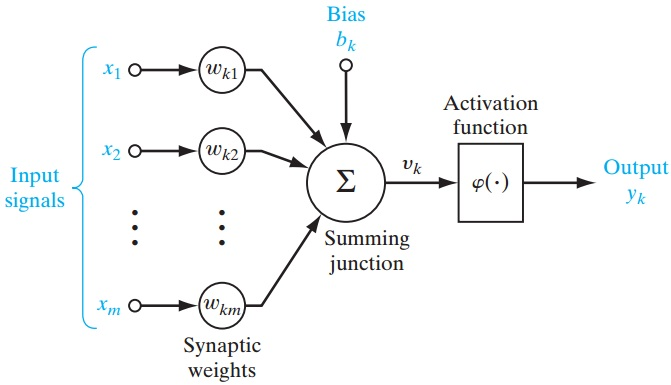
\includegraphics[scale=0.5]{../figures/neurone.jpg}
 \caption{Un neurone artificiel. \textbf{Source}: Haykin\cite{Haykin}}
 \label{neuronemlp}
\end{figure}
Un neurone effectue tout d'abord une somme pondérée de ses entrées \[v_k = b_k+\sum_{j=1}^{m}x_{j}w_{kj}\] où $x$ est le vecteur d'entrée de dimensions $m$.\\
Chaque terme $x_j$ est mutiplié par un poids $w_{kj}$.
Ce sont les poids qui seront modifiés lors de la phase d'apprentissage.
Le biais $b_k$ est souvent ajouté à la pondération.
Mais pour simplifier les formules, nous pouvons considèrer $b_k$ comme étant l'entrée $x_0 = 1$ de poid fixe $w_{k0} = 1$.
Et la somme pondérée est donc maintenant de la forme \[v_k = \sum_{j=0}^{m}x_{j}w_{kj}\]
Ensuite le neurone applique la \emph{fonction d'activation} $\phi$ sur la somme pondérée.
Le domaine de $y$ est généralement $[0,1]$ ou $[-1,1]$.\cite{Haykin,statistica}
La fonction $\phi$ utilisée dépend du problème qu'on veut résoudre (Figure \ref{mlpfonc}).
\begin{figure}
 \centering
 % tableau de statistica
 \textbf{Fonctions d'activations.} (fonction de $x$)\\
 \begin{tabular}{|l|c|c|}
  Nom & Formule & Image\\
  \hline
  Identité & $x$ & $]-\infty,\infty[$\\
  \hline
  Sigmoïde & $\frac{1}{1+\exp^{-x}}$ & $]0,1]$\\
  \hline
  Tangente hyperbolique & $\frac{\exp^{x}-\exp^{-x}}{\exp^{x}+\exp^{-x}}$ & $]-1,1[$\\
  \hline
  Exponentielle & $e^{-x}$ & $]0,\infty[$\\
  \hline
  Sinus & $\sin{x}$ & $[-1,1]$\\
  \hline
  Softmax & $\frac{\exp^{x}}{\sum{\exp^{x_i}}}$ & $]0,1[$\\
  \hline
 \end{tabular}

 \caption{Fonctions d'activation principalement utilisés dans un MLP. \textbf{Source}: STATISTICA Réseaux de Neurones Automatisés (SANN)\cite{statistica}}
 \label{mlpfonc}
\end{figure}
\subsubsection{Structure}
\begin{figure}
 \centering
 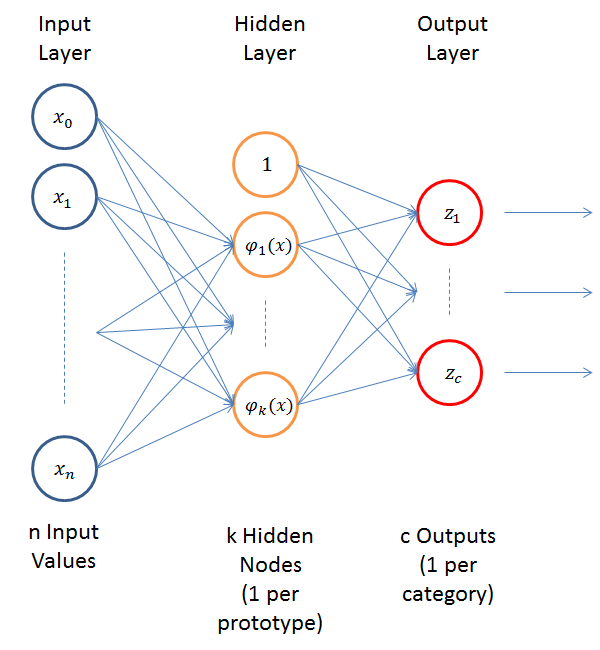
\includegraphics[scale=0.5]{../figures/nnstruct.png}
 \caption{Structure MLP à une couche cachée. \textbf{Source}: McCormick\cite{RBFtuto}}
 \label{structuremlp}
\end{figure}
Un \mlp est composé de plusieurs couches (Figure \ref{structuremlp}):
\begin{center}
 couche d'entrée $\rightarrow$ couches cachées $\rightarrow$ couche de sortie.
\end{center}
Un neurone envoie sa sortie vers tous les neurones de la couche suivante.
Il y a autant de neurones d'entrées que la dimension du vecteur d'entrée.
Le $k$\textsuperscript{ième} neurone d'entrée renvoie juste le $k$\textsuperscript{ième} élément du vecteur d'entrée.
Chaque neurone de sortie correspond à une dimension du vecteur de sortie.
Les neurones cachés et neurones de sortie correspondent à la Figure \ref{neuronemlp}.
\subsubsection{Apprentissage supervisé}\label{sec:appmlp}
Il existe plusieurs algorithmes pour changer les poids sur un réseau. Mais le plus connu est l'algorithme de de rétropropagation.\cite{Haykin,Gauthier}
Il s'agit d'un algorithme d'\emph{apprentissage supervisé}.
\begin{definition}
L'apprentissage supervisé est une méthode visant à améliorer un approximateur grâce à un calcul d'erreur (appelé aussi mesure de performance\cite{Gauthier}) comparant une sortie générée avec la sortie attendue.
\end{definition}
Nous avons donc besoin d'un ensemble de paires d'entrées/sorties.
L'algorithme applique la formule développée ci-dessous à tous les neurones sauf les neurones d'entrée.\\

Soit $\phi_i$, la fonction d'activation du neurone $i$. L'erreur entre la sortie produite et la sortie attendue est donnée par $Q$, l'\emph{erreur quadratique} utilisé comme mesure de performance.
\begin{equation} \label{eq:Q}
 Q = \frac{1}{2}\sum_{i}(\phi_i-s_i)^2
\end{equation}
où $i$ est l'indice d'un neurone de sortie et $s_i$ la sortie attendue pour le neurone $i$.

Nous voulons modifier la valeur des poids pour que la prochaine fois que nous prenons la même entrée, l'erreur $Q$ soit plus petite.
Pour chaque poids $W_{ij}$, nous allons calculer le gradient $\partiel{Q}{W_{ij}}$ qui, par définition, indique la façon dont $Q$ varie si $W_{ij}$ augmente d'une valeur $\delta W_{ij}$ infiniment petite.
Ensuite nous \enum{ferons un pas} dans le sens opposé et proportionel au gradient en ajoutant $-\eta\partiel{Q}{W_{ij}}$ à $W_{ij}$ où $\eta$ est une constante appelé \emph{pas du gradient}.
Donc la modification du poid $W_{ij}$ que nous voulons appliquer vaut
\begin{equation}%\label{eq:Delta}
 \Delta W_{ij} = -\eta\partiel{Q}{W_{ij}}
\end{equation}
Déterminons à présent la valeur de ce gradient $\partiel{Q}{W_{ij}}$.
Nous savons que $\phi_i$ est une équation à une variable.
Mais en entrée de cette variable est donnée la somme pondérée $v_i$ et $W_{ij}$ est un des poids de $v_i$.
Par le théorème de dérivation des fonctions composées,
\begin{equation}%\label{eq:gradient}
 \partiel{Q}{W_{ij}} = \partiel{Q}{\phi_i} \partiel{\phi_i}{v_i} \partiel{v_i}{W_{ij}}
\end{equation}
\begin{thm}[dérivation des fonctions composées]
Soit $f:A~\rightarrow~B : y~\rightarrow~f(y)$ et $g:B~\rightarrow~C : x~\rightarrow~g(x)$. Alors la dérivée de $f~\circ~g$ en $x$ vaut
\[\partiel{f}{x} = \partiel{f}{g} \partiel{g}{x}\]
\end{thm}
Posons
\begin{equation}%\label{eq:deltai}
 \delta_i = \partiel{Q}{\phi_i} \partiel{\phi_i}{v_i}
\end{equation}
$\delta_i$ est appelé \emph{contribution à l'erreur} du neurone $i$.
Nous verrons plus tard qu'elle sera utile pour la rétropropagation de la couche prédédente.
Le dévellopement de la formule de rétropropagation a été fait en annexe \ref{sec:eqmlp}.
Et voici ce que nous obtenons au final:\\
\begin{equation}\label{eq:mlpretro}
 \Delta W_{ij} = -\eta \delta_i x_i \text{~où~}\left\{
  \begin{array}{lll}
   \delta_i & = (\phi_i - s_i)\phi'(v_i) & \text{Si~} i \text{~est un neurone de sortie}\\
   \delta_i & = \phi_i'(v_i) \sum_{k=1}^{n} \delta_k W_{ki} & \text{Si~} i \text{~est un neurone caché}
  \end{array}
 \right.
\end{equation}

\subsubsection{Apprentissage non supervisé}
Il existe également des algorithmes d'apprentissage non supervisé.
Ces algorithmes ne cherchent pas à minimiser une erreur mais maximisent un score calculé à partir de la sortie du réseau.
\subsubsection{Apprentissage sur plusieurs MLP}
Lorque l'une des dimensions du vecteur d'entrée est discrète et finie, il est conseillé d'utiliser un \mlp différent par valeur différente sur cette dimension.\cite{Gauthier}
Cette technique peut aussi être utilisée si nous pouvons classer tous les états possibles selon le contexte.
Par exemple, pour la Sphero nous pourrions utiliser un \mlp pour le contexte \enum{en train de déraper} et un autre \mlp pour le contexte \enum{ne dérape pas}.
\subsubsection{Applications}
À une couche cachée, un \mlp peut déja servir pour la classification non linéaire.\cite{statistica}\\
Les \mlp sont aussi utilisés en commande de robot par caméra.\cite{Pomerleau}
